\documentclass[a4paper, 12pt]{article}
\usepackage[T2A]{fontenc}
\usepackage[utf8]{inputenc}
\usepackage[english,russian]{babel}
\usepackage{amsmath, amsfonts, amssymb, amsthm, mathtools, misccorr, indentfirst, multirow}
\usepackage{wrapfig}
\usepackage{graphicx}
\usepackage{subfig}
\usepackage{adjustbox}
\usepackage{pgfplots}

\usepackage{geometry}
\geometry{top=20mm}
\geometry{bottom=20mm}
\geometry{left=20mm}
\geometry{right=20mm}
\newcommand{\angstrom}{\textup{\AA}}

\title{Лабораторная работа 2.4\\Закон Моззли}
\author{Нехаев Александр, гр. 654}
\date{\today}
\begin{document}
\maketitle
\tableofcontents
\paragraph{Цель работы:}
измерить спектры характеристического излучения атомов для набора химических элементов. Определить рентгеновские термы измеренных спектральных пиков излучения. Проверить закон Мозли. Определить рентгеновские термы измеренных спектральных пиков излучения. Проверить закон Мозли. Определить элементный состав контрольного образца.
\paragraph{В работе используются:}
рентгеновский спектрометр <<Спектроскан Макс-G>>, включающий в себя рентгеновский источник излучения, специально вогнутый кристалл LiF, гониометр, газовый детектор рентгеновских квантов и компьютер, а также образцы чистых химических элементов.
\section{Теоретическое введение}
При переходе электрона с оболочки одного слоя на другой слой атом излучает рентгеновский квант, такое излучение называют характеристическим излучением. Энергия кванта такого излучения приближенно может быть записана в виде:
\begin{equation}
	\hbar\omega_{12}=E_{n_2}-E_{n_1}=-Ry\left(\frac{(Z-\sigma_{n_2,l_2})^2}{n_2^2}-\frac{(Z-\sigma_{n_1,l_1})^2}{n_2^2}\right)
	\label{eq:5}
\end{equation}
где $n_1$ и $n_2$ -- главные квантовые числа конечного и начального состояний электрона. Эта формула является приближённой, причем входящие в нее параметры экранировки заряда ядра $\sigma_{n_2,l_2}$ и $\sigma_{n_1,l_1}$ могут заметно отличаться друг от друга. Это связано с тем, что для электрона, расположенного на заданной электронной оболочке, эффективно экранируют заряд ядра только те электроны, которые распологаются на оболочках меньшего или такого же радиуса. Поэтому для электрона на первой оболочке параметр экранировки составляет величину около единицы (есть еще только один электрон на той же оболочке), а вот для электрона на второй оболочке параметр экранировки будет иметь значение около 7. (Два электрона на первой оболочке и ещё 5 на второй.) Для упрощения формулу (\ref{eq:5}) можно переписать в виде:
\begin{equation}
	\hbar\omega=Ry\cdot\left(Z-\sigma\right)^2\left(\frac{1}{n_1^2}-\frac{1}{n_2^2}\right).
\end{equation}
\par
Это выражение также как и формула (\ref{eq:5}), является приближенным, но оно отражает основное свойство спектральных линий характеристического излучения: квадратичную зависимость частоты излучения от заряда ядра $Z$ -- 
\section{Ход работы}
\subsection{Измерение спектров}
В лабораторной работе предлагается определить длины волн характеристического излучения следующих элементов: $^{22}\text{Ti}$, $^{23}\text{V}$, $^{24}\text{Cr}$, $^{25}\text{Mn}$, $^{26}\text{Fe}$, $^{28}\text{Ni}$, $^{29}\text{Cu}$, $^{41}\text{Nb}$, $^{42}\text{Mo}$, $^{47}\text{Ag}$.\par
Работать будем с наиболее яркими спектральными линиями: $K_{\alpha_{1,2}}$, $K_{\beta_{1,3}}$, $L_{\alpha_1}$, $L_{\beta_1}$.
\subsection{Обработка данных}
\begin{enumerate}
	\item Приведем изображения измеренных спектров:
	\begin{figure}[!htb]
		\minipage{0.3\textwidth}
		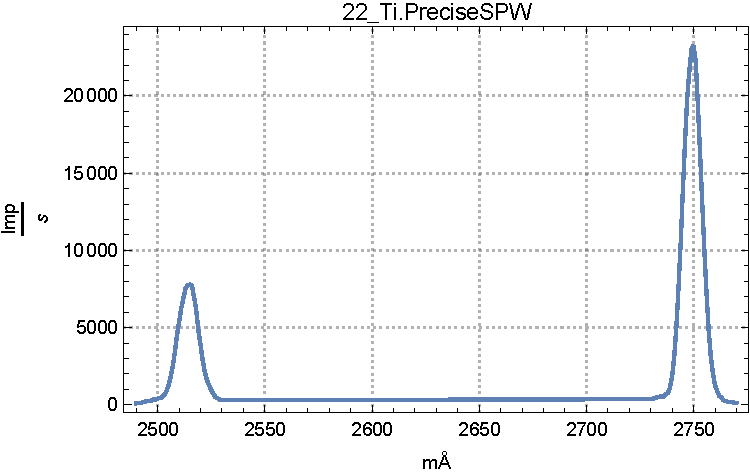
\includegraphics[width=\linewidth]{PhysLab5/22_Ti.PreciseSPW.pdf}
		\caption{Спектр титана}
		\endminipage\hfill
		\minipage{0.3\textwidth}
		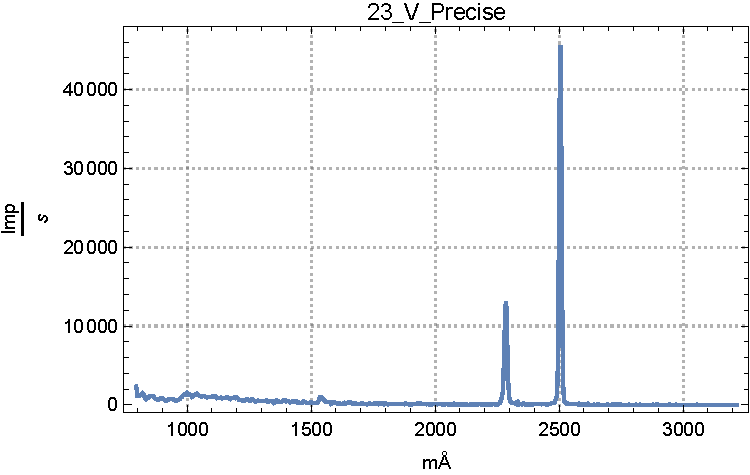
\includegraphics[width=\linewidth]{PhysLab5/23_V_Precise.pdf}
		\caption{Спектр ванадия}
		\endminipage\hfill
		\minipage{0.3\textwidth}
		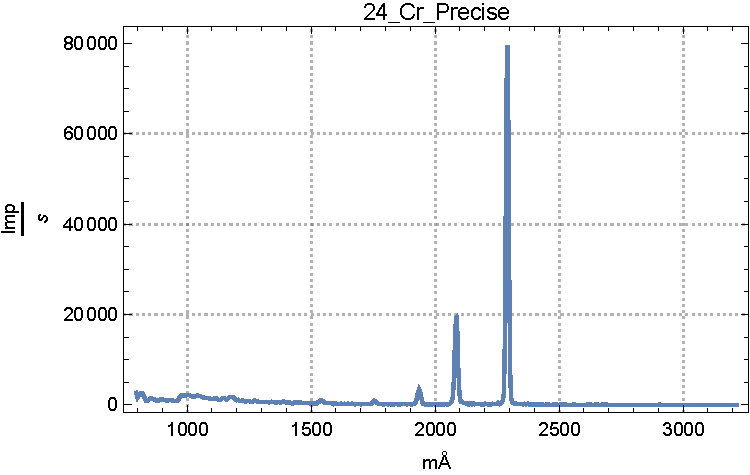
\includegraphics[width=\linewidth]{PhysLab5/24_Cr_Precise.pdf}
		\caption{Спектр хрома}
		\endminipage\hfill
		\minipage{0.3\textwidth}
		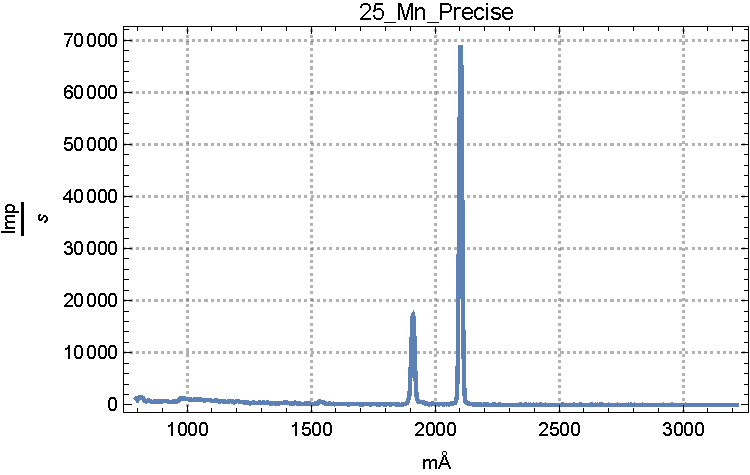
\includegraphics[width=\linewidth]{PhysLab5/25_Mn_Precise.pdf}
		\caption{Спектр марганца}
		\endminipage\hfill
		\minipage{0.3\textwidth}
		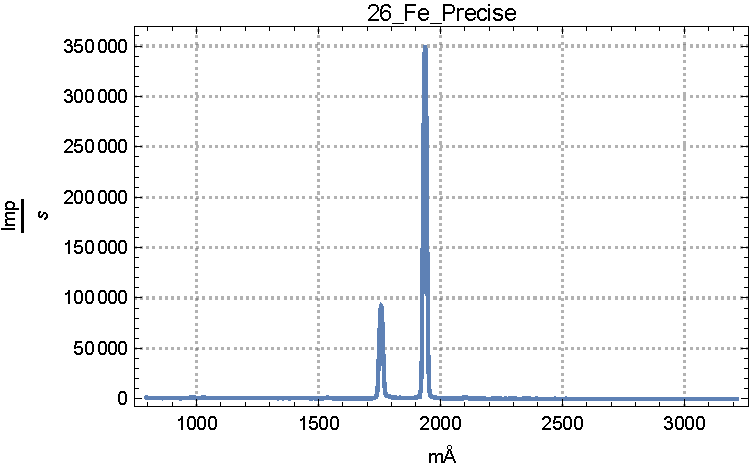
\includegraphics[width=\linewidth]{PhysLab5/26_Fe_Precise.pdf}
		\caption{Спектр железа}
		\endminipage\hfill
		\minipage{0.3\textwidth}
		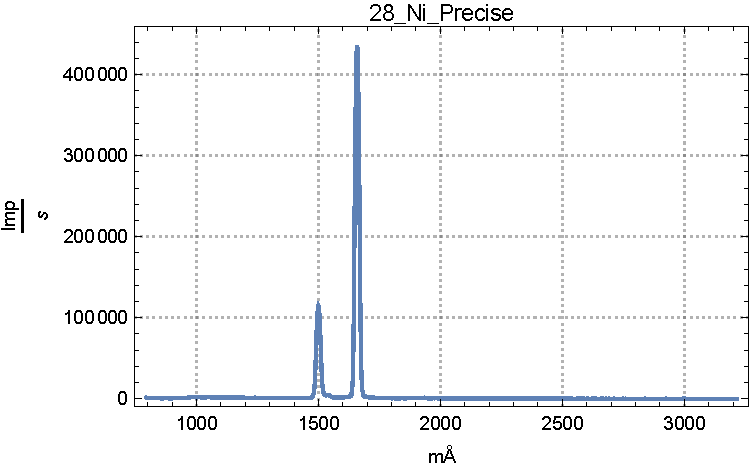
\includegraphics[width=\linewidth]{PhysLab5/28_Ni_Precise.pdf}
		\caption{Спектр никеля}
		\endminipage\hfill
		\minipage{0.3\textwidth}
		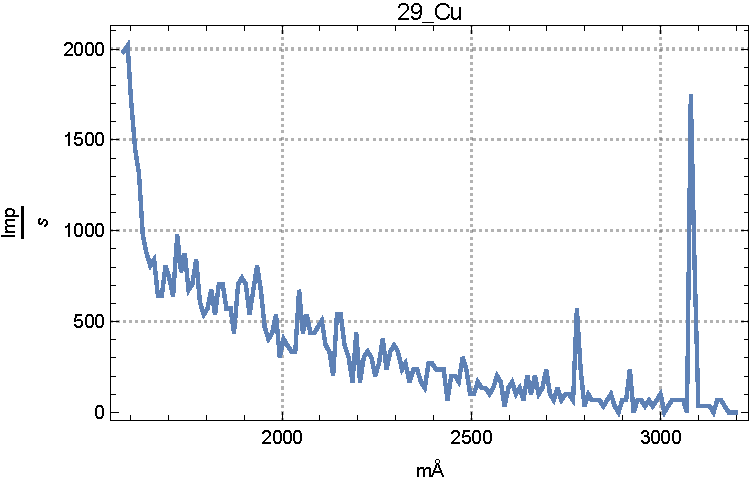
\includegraphics[width=\linewidth]{PhysLab5/29_Cu.pdf}
		\caption{Спектр меди}
		\endminipage\hfill
		\minipage{0.3\textwidth}
		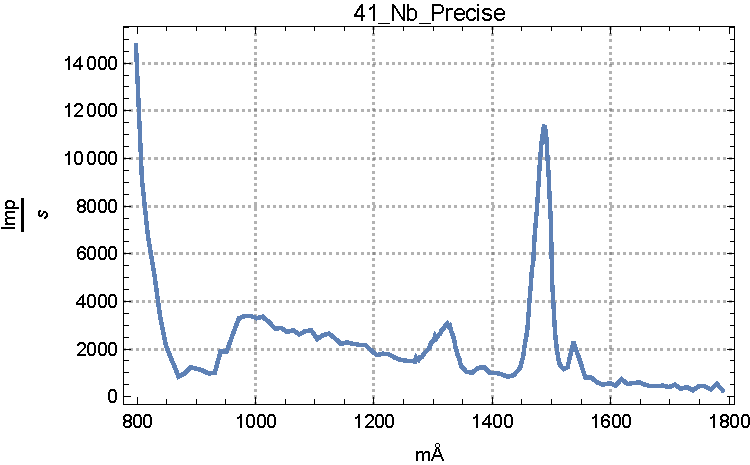
\includegraphics[width=\linewidth]{PhysLab5/41_Nb_Precise.pdf}
		\caption{Спектр ниобия}
		\endminipage\hfill
		\minipage{0.3\textwidth}
		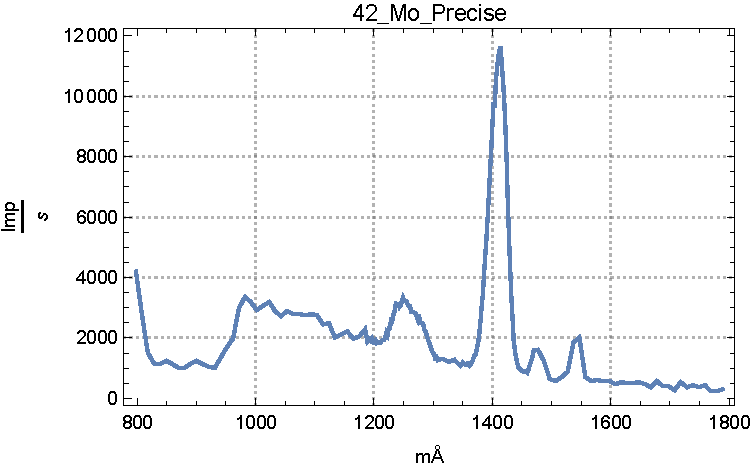
\includegraphics[width=\linewidth]{PhysLab5/42_Mo_Precise.pdf}
		\caption{Спектр молибдена}
		\endminipage\hfill
		\minipage{0.3\textwidth}
		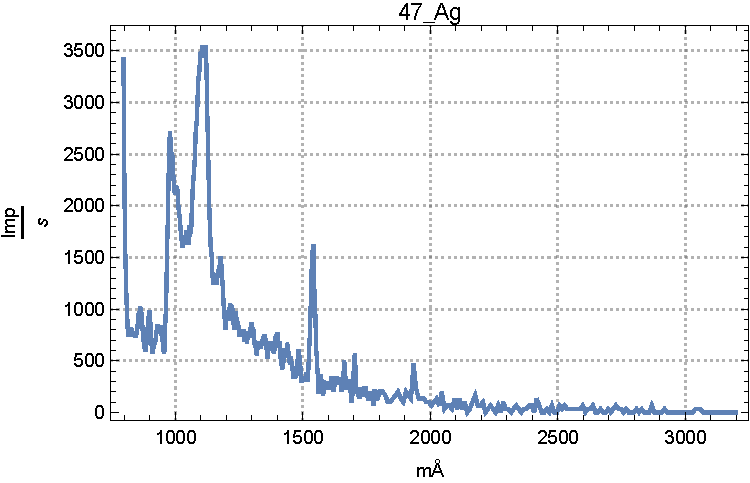
\includegraphics[width=\linewidth]{PhysLab5/47_Ag.pdf}
		\caption{Спектр серебра}
		\endminipage\hfill
		\minipage{0.3\textwidth}
		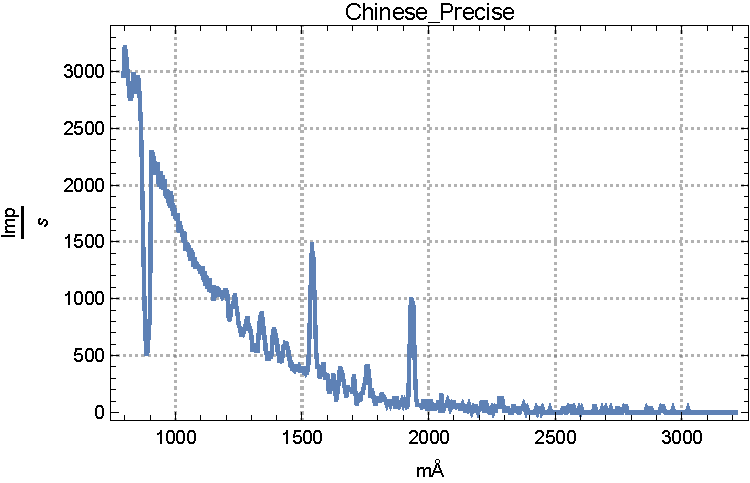
\includegraphics[width=\linewidth]{PhysLab5/Chinese_Precise.pdf}
		\caption{Спектр китайской монетки}
		\endminipage\hfill
	\end{figure}
	\item На основе измеренных данных составим таблицу:
	\newpage
	\begin{table}[!htb]
		\centering
		\caption{Экспериментальные данные}
		\begin{tabular}{|c|c|c|c|c|c|c|c|}
			\hline
			Элемент & Z & $\lambda _{K_{\alpha }}$ & $\lambda _{K_{\beta }}$ & $E_{K_{\alpha}}$ & $E_{K_{\beta }}$ & $\sqrt{\frac{E_{K_{\alpha}}}{\text{Ry}}}$ & $\sqrt{\frac{E_{K_{\beta}}}{\text{Ry}}}$ \\
			\hline
   			Ti & 22 & $2749.9\text{ m{\AA}}$ & $2514.9\text{ m{\AA}}$ & $4508.53\text{ eV}$ & $4929.82\text{ eV}$ & 18.2036 & 19.0351 \\
   			V & 23 & $2505\text{ m{\AA}}$ & $2285\text{ m{\AA}}$ & $4949.3\text{ eV}$ & $5425.82\text{ eV}$ & 19.0727 & 19.9697 \\
   			Cr & 24 & $2291.1\text{ m{\AA}}$ & $2086\text{ m{\AA}}$ & $5411.37\text{ eV}$ & $5943.43\text{ eV}$ & 19.9431 & 20.9006 \\
   			Mn & 25 & $2104\text{ m{\AA}}$ & $1911.\text{ m{\AA}}$ & $5892.59\text{ eV}$ & $6487.7\text{ eV}$ & 20.811 & 21.8366 \\
   			Fe & 26 & $1937\text{ m{\AA}}$ & $1757\text{ m{\AA}}$ & $6400.62\text{ eV}$ & $7056.35\text{ eV}$ & 21.6896 & 22.7735 \\
   			Ni & 28 & $1658\text{ m{\AA}}$ & $1500.1\text{ m{\AA}}$ & $7477.68\text{ eV}$ & $8264.78\text{ eV}$ & 23.4435 & 24.6465 \\
			Cu & 29 & $1540\text{ m{\AA}}$ & $1390\text{ m{\AA}}$ & $8050.65\text{ eV}$ & $8919.42\text{ eV}$ & 24.3251 & 25.604 \\
			Ag & 47 & $560\text{ m{\AA}}$ & $500\text{ m{\AA}}$ & $22139.3\text{ eV}$ & $24796.\text{eV}$ & 40.3387 & 42.6904 \\
			Mo & 42 & $711\text{ m{\AA}}$ & $632\text{ m{\AA}}$ & $17437.4\text{ eV}$ & $19617.1\text{ eV}$ & 35.7998 & 37.9714 \\
			Nb & 41 & $748\text{ m{\AA}}$ & $666\text{ m{\AA}}$ & $16574.9\text{ eV}$ & $18615.6\text{ eV}$ & 34.9032 & 36.9895 \\
			\hline
		\end{tabular}
	\end{table}
	\item Для всех спектральных линий построим на одном графике зависимости величины $\sqrt{\frac{E}{Ry}}$ от атомного номера $Z$.
	\begin{figure}[!htb]
	\label{graph}
	\begin{tikzpicture}
		\begin{axis}[
		xlabel=Z,
		ylabel=$\sqrt{\frac{E}{Ry}}$,
		xmin=22,
		xmax=47,
		ymin=17,
		ymax=43,
		ymajorgrids=true,
		xmajorgrids=true,
    	grid style= dashed,
    	width=\textwidth,
    	]
    	\addplot[
    	color=black,
		mark=square,
		only marks,
    	]
    	coordinates{
    	(22, 18.2036)
    	(23, 19.0727)
    	(24, 19.9431)
    	(25, 20.811)
    	(26, 21.6896)
    	(28, 23.4435)
    	(29, 24.3251)
    	(41, 34.9032)
    	(42, 35.7998)
    	(47, 40.3387)
    	};
    	\addplot[
    	color=black,
		mark=square,
		only marks,
    	]
    	coordinates{
    	(22, 19.0351)
    	(23, 19.9697)
    	(24, 20.9006)
    	(25, 21.8366)
    	(26, 22.7735)
    	(28, 24.6465)
    	(29, 25.604)
    	(41, 36.9895)
    	(42, 37.9714)
    	(47, 42.6904)
    	};
    	\addplot[
    	domain=22:47,
		samples=3,
		color=black
    	]
    	{-1.27391+0.883614*x};
    	\addplot[
    	domain=22:47,
		samples=3,
		color=black
    	]
    	{-1.84261+0.947373*x};
		\end{axis}
	\end{tikzpicture}
	\caption{График зависимости $\sqrt{\frac{E_K}{Ry}}$ от $Z$}
	\end{figure}
	\par
	Параметры аппроксимации:
	\begin{equation*}
		y=(-1.27391\pm 0.04955)+(0.883614\pm 0.001553)x
	\end{equation*}
	\begin{equation*}
		y=(-1.84261\pm 0.029109)+(0.947373\pm 0.000912)x
	\end{equation*}
	\item Используя формулу и полученные графики зависимости, определим постоянные $\sigma$ и $\left(\frac{1}{n_1^2}-\frac{1}{n_2^2}\right)$
	\begin{equation*}
		\sqrt{\frac{E}{Ry}}=(Z-\sigma)\sqrt{\left(\frac{1}{n_1^2}-\frac{1}{n_2^2}\right)}=Z\sqrt{\left(\frac{1}{n_1^2}-\frac{1}{n_2^2}\right)}-\sigma\sqrt{\left(\frac{1}{n_1^2}-\frac{1}{n_2^2}\right)}=Zb+a
	\end{equation*}
	\begin{equation*}
		b=\sqrt{\left(\frac{1}{n_1^2}-\frac{1}{n_2^2}\right)}
	\end{equation*}
	\begin{equation*}
		\sigma=-\frac{a}{b}
	\end{equation*}
	Таким образом получили константы экранирования:
	\begin{equation*}
		\sigma_{K_\alpha}=1.44171
	\end{equation*}
	\begin{equation*}
		\sigma_{K_\beta}=1.94497
	\end{equation*}
\end{enumerate}
\end{document}